%\documentclass[12pt,a4paper]{report}
%\usepackage[utf8]{inputenc}
%\usepackage{amsmath}
%\usepackage{amsfonts}
%\usepackage{amssymb}
%\usepackage[margin=2.5cm]{geometry}
%\usepackage{graphicx}
%\usepackage{caption}
%\usepackage{subcaption}
%\usepackage[nottoc,numbib]{tocbibind}
%\linespread{1.3}
%\begin{document}
\chapter{Rectangular Barrier}
\label{Rectangular Barrier}
	In this section the transport properties for massive Dirac fermions through a potential barrier will be examined. This problem was originally studied with respect to potential barriers \cite{b12}, but has been expanded to include magnetic field \cite{b14} and energy gaps \cite{b4,b13,b15,b16,b17}. The massive rectangular potential barrier can be split into seven transmission regions shown in Figure \ref{rectangular-barrier-regions-flat} (a) and three different wave-function regions shown in Figure \ref{rectangular-barrier-regions-flat} (b). The first region of transport in Figure \ref{rectangular-barrier-regions-flat} (a) is below the Fermi level therefore only hole transport exists; transmission, reflection, resonances and Klein tunnelling can occur here. In region 2 $\hbar v_{f}k_{y}$ is larger than energy $E$, this is a region of hole transport shifted by the potential into a non-valid energy region allowing bound states to occur within the barrier but decay outside. Region 3 shows electron-hole transport within the potential barrier, pure oscillatory solutions provide similar properties to region 1. Region 4 is a region of no propagation that has been shifted by the potential. Energy is no longer less than $\hbar v_{f}k_{y}$, however, it maintains the properties of a region of no propagation. This region is responsible for the drop in transmission probability at $E\approx V$. Region 5 is above the barrier, pure electron transport again shows similar properties to region 1. In region 6 energy is less than $\hbar v_{f}k_{y}$, therefore no propagation can occur here. For massive quasiparticles the 7th region must be included, here the energy gap introduces extra regions of no propagation caused by the gap in the energy spectrum before and inside the barrier. These seven regions can then be applied to Figure \ref{rectangular-barrier-regions-flat} (b); region 1 occurs at energies below zero energy, regions 2, 3 occurs within the barrier, region 4 is  located where energy is close to barrier height, region 5 occurs above the barrier and region 7 is between the gaps in the energy spectrum. As the energy $E$ cannot be lower than $\hbar v_{f}k_{y}$ region 6 cannot be shown on Figure \ref{rectangular-barrier-regions-flat} (b).
\begin{figure}
	\begin{subfigure}{0.45\textwidth}
		\centerline{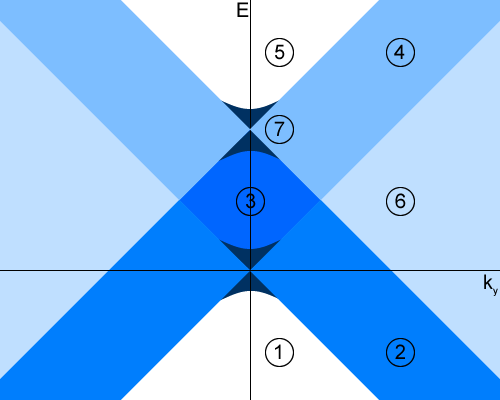
\includegraphics[scale=0.4]{images/rectangular-barrier-regions-flat}}
		\caption{}
	\end{subfigure}
	\hspace{1.2cm}
	\begin{subfigure}{0.45\textwidth}
		\centerline{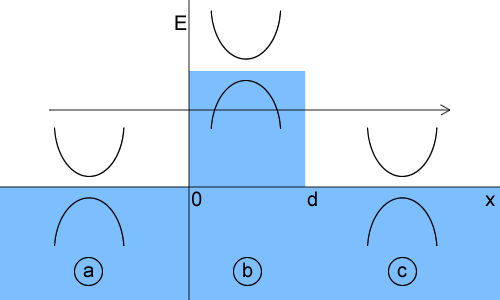
\includegraphics[scale=0.45]{images/potential-constant-mass-barrier-flat}}
		\caption{}
	\end{subfigure}
	\caption{(a) The seven independent regions of transmission for massive quasiparticles in a potential barrier. Six regions exist for a massless graphene potential barrier. The seventh region is caused by the introduction of an energy gap into the graphene spectrum. (b) The three wave-function regions a, b and c for massive quasiparticles in a potential barrier. Also shown is the parabolic dispersion relation and band gap caused by an energy gap in the graphene Hamiltonian.}
	\label{rectangular-barrier-regions-flat}
\end{figure}
%%%%%
%%%%%
%%%%%
	\section{Transfer Matrix}
	\label{Rectangular Barrier - Transfer Matrix}
		This section shows the transfer matrix method for solving the massive rectangular potential barrier. Oscillatory wave-functions with mass and potential will be used in all three regions. The subscript lettering for $q, \theta, V, m$ and $\alpha$ has been introduced to seperate constants in the corresponding barrier regions in Figure \ref{rectangular-barrier-regions-flat} (b). The normalised wave-functions in regions $a,b$ and $c$ can be taken from Section \ref{Wave-functions - Oscillitary}:
			\begin{align}
				\psi\left(x,y\right)_{a,b,c}=
				c_{a,b,a}e^{ik_{y}y}
				\left[\begin{array}{ccc}
					e^{iq_{a,b,a}x}&e^{-iq_{a,b,a}x}\\
					\alpha_{a,b,a}e^{iq_{\left(a,b,a\right)}x+i\theta_{a,b,a}}&-\alpha_{a,b,a}e^{-iq_{a,b,a}x-i\theta_{a,b,a}}
				\end{array}\right]
				\left[\begin{array}{ccc}
					a_{1,3,5}\\
					a_{2,4,6}
				\end{array}\right]
			\end{align}
			The continuity of wave-functions requires that at the first barrier interface $x=d_{1}$, the wave-function $\psi_{a}$ must be equal to $\psi_{b}$. In matrix form this can be written as:
			\begin{align}
				c_{a}
				\left[\begin{array}{ccc}
					e^{iq_{a}d_{1}}&e^{-iq_{a}d_{1}}\\
					\alpha_{a}e^{iq_{a}d_{1}+i\theta_{a}}&-\alpha_{a}e^{-iq_{a}d_{1}-i\theta_{a}}
				\end{array}\right]
				\left[\begin{array}{ccc}
					a_{1}\\
					a_{2}
				\end{array}\right]
				&=
				c_{b}
				\left[\begin{array}{ccc}
					e^{iq_{b}d_{1}}&e^{-iq_{b}d_{1}}\\
					\alpha_{b}e^{iq_{b}d_{1}+i\theta_{b}}&-\alpha_{b}e^{-iq_{b}d_{1}-i\theta_{b}}
				\end{array}\right]
				\left[\begin{array}{ccc}
					a_{3}\\
					a_{4}
				\end{array}\right]
			\end{align}
			For simplicity the matrices $m_{1}$ and $m_{2}$ have been introduced to represent the wave-functions on either side of the interface so that:
			\begin{align}
				m_{1}\left[\begin{array}{ccc}
					a_{1}\\
					a_{2}
				\end{array}\right]
				&=
				m_{2}\left[\begin{array}{ccc}
					a_{3}\\
					a_{4}
				\end{array}\right]
			\end{align}
			At the second barrier interface $x=d_{2}$, continuity requires that $\psi_{b}$ must be equal to $\psi_{c}$:
			\begin{align}
				c_{b}
				\left[\begin{array}{ccc}
					e^{iq_{b}d_{2}}&e^{-iq_{b}d_{2}}\\
					\alpha_{b}e^{iq_{b}d_{2}+i\theta_{b}}&-\alpha_{b}e^{-iq_{b}d_{2}-i\theta_{b}}
				\end{array}\right]
				\left[\begin{array}{ccc}
					a_{3}\\
					a_{4}
				\end{array}\right]
				&=
				c_{a}
				\left[\begin{array}{ccc}
					e^{iq_{a}d_{2}}&e^{-iq_{a}d_{2}}\\
					\alpha_{a}e^{iq_{a}d_{2}+i\theta_{a}}&-\alpha_{a}e^{-iq_{a}d_{2}-i\theta_{a}}
				\end{array}\right]
				\left[\begin{array}{ccc}
					a_{5}\\
					a_{6}
				\end{array}\right]
			\end{align}
			Here $m_{3}$ and $m_{4}$ will be introduced to represent the wave-functions on either side of the barrier interface so that:
			\begin{align}
				m_{3}\left[\begin{array}{ccc}
					a_{3}\\
					a_{4}
				\end{array}\right]
				&=
				m_{4}\left[\begin{array}{ccc}
					a_{5}\\
					a_{6}
				\end{array}\right]
			\end{align}
			With these matrices the constants $a_{3}$ and $a_{4}$ can be removed and the transfer matrix $M$ becomes:
			\begin{align}
				\left[\begin{array}{ccc}
					a_{5}\\
					a_{6}
				\end{array}\right]=M
				\left[\begin{array}{ccc}
					a_{1}\\
					a_{2}
				\end{array}\right]\hspace{1cm}
				M=m_{4}^{-1}m_{3}m_{2}^{-1}m_{1}
			\end{align}
			The barrier interfaces can be set to $d_{1}=0$ and $d_{2}=d$ to produce the matrix elements:
				\begin{align}
					M_{1,1}&=\frac{e^{-iq_{a}d}\left(2\alpha_{a}\alpha_{b}\cos(\theta_{a})\cos(\theta_{b})\cos(q_{b}d)-i\sin(q_{b}d)\left(2\alpha_{a}\alpha_{b}\sin(\theta_{a})\sin(\theta_{b})-\alpha_{a}^{2}-\alpha_{b}^{2}\right)\right)}{2\alpha_{a}\alpha_{b}\cos(\theta_{a})\cos(\theta_{b})}\\
					M_{1,2}&=\frac{e^{-iq_{a}d}2i\sin(q_{b}d)\left(\alpha_{b}^{2}-\alpha_{a}\alpha_{b}e^{-i\theta_{a}}2i\sin(\theta_{b})-\alpha_{a}^{2}e^{-2i\theta_{a}}\right)}{2\alpha_{a}\alpha_{b}\cos(\theta_{a})\cos(\theta_{b})}\\
					M_{2,1}&=-\frac{e^{iq_{a}d}2i\sin(q_{b}d)\left(\alpha_{b}^{2}+\alpha_{a}\alpha_{b}e^{-i\theta_{a}}2i\sin(\theta_{b})-\alpha_{a}^{2}e^{-2i\theta_{a}}\right)}{2\alpha_{a}\alpha_{b}\cos(\theta_{a})\cos(\theta_{b})}\\
M_{2,2}&=\frac{e^{iq_{a}d}\left(2\alpha_{a}\alpha_{b}\cos(\theta_{a})\cos(\theta_{b})\cos(q_{b}d)+i\sin(q_{b}d)\left(2\alpha_{a}\alpha_{b}\sin(\theta_{a})\sin(\theta_{b})-\alpha_{a}^{2}-\alpha_{b}^{2}\right)\right)}{2\alpha_{a}\alpha_{b}\cos(\theta_{a})\cos(\theta_{b})}
				\end{align}
				This transfer matrix satisfies all of the following properties \cite{b18}, which shows that the transfer matrix is valid.
				\begin{align}
					\det(M)=1\hspace{1cm}M_{1,1}=M_{2,2}^{*}\hspace{1cm}M_{1,2}=M_{2,1}^{*}
				\end{align}
				Using this matrix the transmission coefficient can easily be found as it is known that the constants have the following values: $a_{1}=1, a_{2}=r, a_{3}=t$ and $a_{4}=0$
				\begin{align}
					\left[\begin{array}{ccc}
						t\\
						0
					\end{array}\right]=
					\left[\begin{array}{ccc}
						M_{11}&M_{12}\\
						M_{21}&M_{22}
					\end{array}\right]
					\left[\begin{array}{ccc}
						1\\
						r
					\end{array}\right]\hspace{1cm}
					t=\frac{1}{M_{22}}\hspace{1cm}T=|t|^{2}
				\end{align}
				Then the transmission probability $T$ can be calculated as:
				\begin{equation}
					T=\frac{4\alpha_{a}^{2}\alpha_{b}^{2}\cos^{2}(\theta_{a})\cos^{2}(\theta_{b})}{4\alpha_{a}^{2}\alpha_{b}^{2}\cos^{2}(q_{b}d)\cos^{2}(\theta_{a})\cos^{2}(\theta_{b})+\sin^{2}(q_{b}d)\left(2\alpha_{a}\alpha_{b}\sin(\theta_{a})\sin(\theta_{b})-\alpha_{a}^{2}-\alpha_{b}^{2}\right)^{2}}
					\label{eq:transmission}
				\end{equation}
				This result includes an energy gap and potential term. If the respective energy gap, or potential term is set to zero the results in \cite{b1} can be obtained. When potentials approach the electron mass $V \approx m_{e}c^{2}$ \cite{b49}, $\theta_{b}\rightarrow 0$ and the transmission probability reduces to the result for Klein tunnelling shown in \cite{b12}:
				\begin{equation}
					T=\frac{\cos^{2}(\theta_{a})}{1-\cos^{2}(q_{b}d)\sin^{2}(\theta_{a})}
					\label{t2}
				\end{equation}
				The result in Equation (\ref{eq:transmission}) is then plotted in Figure \ref{transmissionplot}. This result can be reduced to the graphene potential barrier in Figure \ref{transmissionplot} (a), a region of finite mass in Figure \ref{transmissionplot} (b) or the massive potential barrier shown in Figure \ref{transmissionplot} (c). The potential barrier features $T=1$ when $\theta_{a}=0$ for all energies with exception of $E=V_{a,b}$ and shows clear resonances. The introduction of a region of finite mass creates a region of no propagation centered at $E=0$, with symmetrical transmission probability outside of this gap. The massive potential barrier shows properties of both of these cases, the asymetrical transmission probability on the energy axis from the potential barrier and the regions of no propagation from the region of finite mass. Under the condition of Klein tunnelling ($V\approx m_{e}c^{2}$) all of these barriers experience perfect transmission with the exception of inside the gap regions. Inside the gap regions the transmission probability approaches zero but sharply increases to one outside.
\begin{figure}
	\begin{subfigure}{0.3\textwidth}
		\centerline{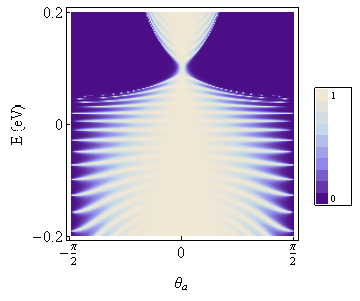
\includegraphics[scale=0.43]{images/potential}}
		\caption{$m_{a,b}=0$ eV and $V_{b}=0.1$ eV.}
	\end{subfigure}
	\hspace{0.5cm}
	\begin{subfigure}{0.3\textwidth}
		\centerline{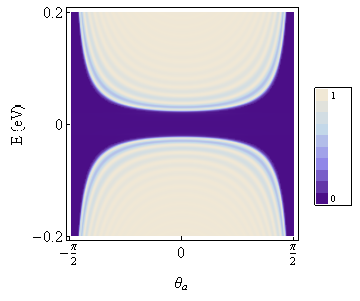
\includegraphics[scale=0.43]{images/mass}}
		\caption{$m_{a}=0$ eV, $m_{b}=0.02$ eV and $V_{b}=0$ eV.}
	\end{subfigure}
	\hspace{0.5cm}
	\begin{subfigure}{0.3\textwidth}
		\centerline{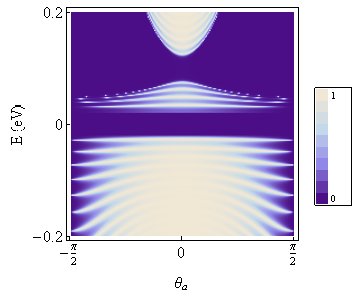
\includegraphics[scale=0.43]{images/transmission}}
		\caption{$m_{a,b}=0.02$ eV and $V_{b}=0.1$ eV.}
	\end{subfigure}
	\caption{Density plots of transmission probability $T$ against energy $E$ and incident angle $\theta_{a}$ from Equation (\ref{eq:transmission}). In all plots the width $d=200$ nm and $V_{a}=0$ eV. (a) Shows results for the potential barrier with gapless Dirac spectrum. (b) Massless Dirac fermions entering a region of finite mass. (c) Massive quasiparticles transmit through a potential barrier.}
	\label{transmissionplot}
\end{figure}

				In Figure \ref{thinbarrier} (a) the transmission probability is plotted with the depenence on energy gap. At larger values of energy gap it can be seen that the gap region increases fairly linearly, however at small energy gaps there is a non-negligible transmission probability. Similarly in Figure \ref{thinbarrier} (b) the dependence of barrier width on transmission probability is shown. Here as width increases the number of resonances increases. For thin barriers a finite transmission probability occurs at all energies, again removing the effect of the energy gap.
\begin{figure}
	\begin{subfigure}{0.45\textwidth}
		\centerline{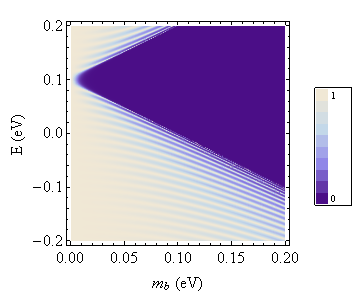
\includegraphics[scale=0.5]{images/contour-t-m}}
		\caption{$m_{a}=0$ eV, $V_{a}=0$ eV, $V_{b}=0.1$ eV and $d=200$ nm.}
	\end{subfigure}
	\hspace{1.2cm}
	\begin{subfigure}{0.45\textwidth}
		\centerline{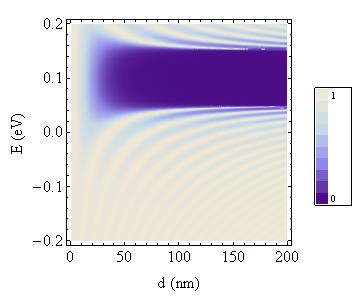
\includegraphics[scale=0.5]{images/mass-potential-e-d}}
		\caption{$m_{b}=0.05$ eV, $m_{a}=0$ eV, $V_{a}=0$ eV and $V_{b}=0.1$ eV.}
	\end{subfigure}
	\caption{Density plots of transmission probability against energy gap and barrier width. In (a) The transmission properties with a varying energy gap. (b) The dependence of barrier width $d$ on the transmission probability.}
	\label{thinbarrier}
\end{figure}
%%%%%
%%%%%
%%%%%
			\section{Fabry-P\'{e}rot Resonances}
			\label{Rectangular Barrier - Fabry-Perot Resonances}
				A single graphene barrier can act as a Fabry-P\'{e}rot resonator \cite{b38}. At resonance the transmission probability $T$ will be equal to one. It is clear from Equation (\ref{eq:transmission}) that this requirement is met when $q_{b}d=n\pi$. Evaluating this relation provides the energies where the Fabry-P\'{e}rot resonances can be found.
				\begin{equation}
					E=V_{b}\pm\sqrt{\hbar^{2}v_{f}^{2}\left(\frac{n^{2}\pi^{2}}{d^{2}}+k_{y}^{2}\right)+m_{b}^{2}}
					\label{resonances-barrier}
				\end{equation}
				The condition of $E=\hbar v_{f}k_{y}$ is the limit of where real solutions exist. This condition can be applied to Equation (\ref{resonances-barrier}), which then becomes:
				\begin{equation}
					E=\frac{V_{b}}{2}-\frac{v_{f}^{2}\hbar^{2}n^{2}\pi^{2}+d^{2}m_{b}^{2}}{2V_{b}d^{2}}
				\end{equation}
	Showing the energies at which real and imaginary solutions coincide. When an energy gap is introduced the gap centered around $V_{b}$ increases by $2m$. This increased gap reduces the energy region resonances can exist, resulting in a higher density of resonances. If the energy gap $m_{b}=0$ this result can be reduced to the gapless case in \cite{b14}. These resonances are not restricted to potential barriers; for the case of $V_{a,b}=0$, $m_{a}=0$ and $m_{b} \neq 0$ resonances can still be obtained.
\begin{figure}
	\centerline{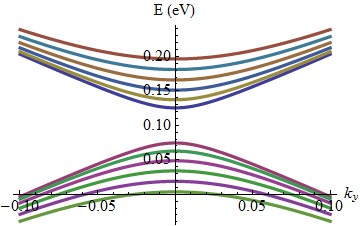
\includegraphics[scale=0.5]{images/mass-potential-energy-levels}}
	\label{}
	\caption{The dependence of energy $E$ and $k_{y}$ on Fabry-P\'{e}rot resonances as described by Equation (\ref{resonances-barrier}) with $\hbar v_{f}=1$. Here the barrier has the properties $m_{a,b}=0.02$ eV, $V_{b}=0.1$ eV, $V_{a}=0$ eV and width $d=200$ nm.}
\end{figure}
%%%%%
%%%%%
%%%%%
			\section{Bound States}
			\label{Rectangular Barrier - Bound States}
				A bound state will only be found within a barrier, therefore the wave-functions must decay outside of the barrier. To find the bound states within a potential barrier the wave-function system of growth-oscillatory-decay shown in Figure \ref{bound-states} is needed. Using the wave-functions derived in Section \ref{Wave-functions - Growth and Decay} and Section \ref{Wave-functions - Oscillitary} this system can be constructed. The wave-functions in each region take the form:
				\begin{align}
					\psi_{a}=a_{1}
					\left[\begin{array}{ccc}
						e^{q_{d}x}\\
						i\alpha_{-}e^{q_{d}x}
					\end{array}\right]e^{ik_{y}y}
				\end{align}
				\begin{align}
					\psi_{b}=
					\left[\begin{array}{ccc}
						e^{iqx}&e^{-iqx}\\
						\alpha e^{iqx+i\theta}&-\alpha e^{-iqx-i\theta}
					\end{array}\right]
					\left[\begin{array}{ccc}
						a_{2}\\
						a_{3}
					\end{array}\right]e^{ik_{y}y}
				\end{align}
				\begin{align}
					\psi_{c}=a_{4}
					\left[\begin{array}{ccc}
						e^{-q_{d}x}\\
						-i\alpha_{+}e^{-q_{d}x}
					\end{array}\right]e^{ik_{y}y}
				\end{align}
				At the boundaries $d_{1}$ and $d_{2}$ the continuity of wave-functions requires that $\psi_{a}=\psi_{b}$ and $\psi_{b}=\psi_{c}$. From this condition the set of simultaneous equations can be made:
				\begin{align}
					a_{1}e^{q_{d}d_{1}}&=a_{2}e^{iqd_{1}}+a_{3}e^{-iqd_{1}}\\
					-ia_{1}\alpha_{-}e^{q_{d}d_{1}}&=\alpha\left(a_{2}e^{iqd_{1}+i\theta}-a_{3}e^{-iqd_{1}-i\theta}\right)\\
					a_{2}e^{iqd_{2}}+a_{3}e^{-iqd_{2}}&=a_{4}e^{-q_{d}d_{2}}\\
					\alpha\left(a_{2}e^{iqd_{2}+i\theta}-a_{3}e^{-iqd_{2}-i\theta}\right)&=ia_{4}\alpha_{+}e^{-q_{d}d_{2}}
				\end{align}
				Re-arranging these to be equal to zero the matrix $m$ can be made:
				\begin{align}
					\left[\begin{array}{cccc}
						e^{q_{d}d_{1}}&-e^{iqd_{1}}&-e^{-iqd_{1}}&0\\
						-i\alpha_{-}e^{q_{d}d_{1}}&-\alpha e^{iqd_{1}+i\theta}&\alpha e^{-iqd_{1}-i\theta}&0\\
						0&e^{iqd_{2}}&e^{-iqd_{2}}&-e^{-q_{d}d_{2}}\\
						0&\alpha e^{iqd_{2}+i\theta}&-\alpha e^{-iqd_{2}-i\theta}&-i\alpha_{+}e^{-q_{d}d_{2}}\\
					\end{array}\right]
					\left[\begin{array}{cccc}
						a_{1}\\
						a_{2}\\
						a_{3}\\
						a_{4}\\
					\end{array}\right]=
					\left[\begin{array}{cccc}
						0\\
						0\\
						0\\
						0\\
					\end{array}\right]
				\end{align}
				To find non-trivial solutions set $\det(m)=0$, $d_{1}=0$ and $d_{2}=d$. From this the dispersion relation can be found:
				\begin{equation}
					\tan(qd)=-\frac{q_{d}q}{\frac{E^{2}-m_{a}m_{b}+V_{a}V_{b}-E\left(V_{a}+V_{b}\right)}{\hbar^{2}v_{f}^{2}}-k_{y}^{2}}
					\label{boundstates}
				\end{equation}
				When the energy gap is removed this result can be reduced to the results for the potential barrier with a Dirac spectrum shown in \cite{b3}. The effect of the energy gap on the bound states is similar that of the Fabry-P\'{e}rot resonances; the energy gap reduces the valid region for bound states to exist, which causes the peaks of the states to occur at lower energies within the barrier. If the energy gap is significantly large, states at higher energies may be lost until the valid energy region approaches zero.
\begin{figure}
	\begin{subfigure}{0.45\textwidth}
		\centerline{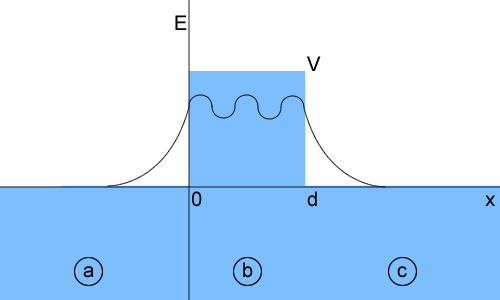
\includegraphics[scale=0.4]{images/bound-states}}
		\caption{}
		\label{}
	\end{subfigure}
	\hspace{1.2cm}
	\begin{subfigure}{0.45\textwidth}
		\centerline{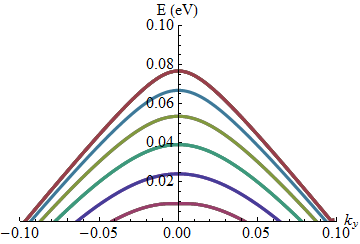
\includegraphics[scale=0.7]{images/bound-states-plot}}
		\caption{}
		\label{}
	\end{subfigure}
	\caption{(a) The required wave-function system to find bound states within a potential barrier. (b) The bound states found from Equation (\ref{boundstates}) within a potential barrier with massive quasiparticles where $\hbar v_{f}=1$, $m_{a,b}=0.02$ eV, $V_{b}=0.1$ eV, $V_{a}=0$ eV and the width $d=200$ nm.}
	\label{bound-states}
\end{figure}
%%%%%
%%%%%
%%%%%
		\section{Conductance}
		\label{Rectangular Barrier - Conductance}
	The conductance through a device can then be calculated via the Landauer formalism as described in Section \ref{Introduction - Landauer Formalism in Graphene}. In Figure \ref{pot-g-1} the conductance has been plotted against the Fermi level of the system. Experimentally this would be adjusted by applying a gate voltage to the substrate of the device \cite{b46}. In Figure \ref{pot-g-1} (a) and Figure \ref{pot-g-1} (b) the same barrier has been plotted at low temperature and at room temperature. It can be seen that the barrier creates minima at zero energy and at barrier height. Outside of the barrier region, the conductance becomes linear due to the graphene density of states. When the temperature is increased in Figure \ref{pot-g-1} (b) the barrier region smooths out reducing the effect of the potential. In Figure \ref{pot-g-1} (c) a small energy gap is included at zero and at barrier height, this creates regions of zero conductance centered at zero energy and at barrier height.
		\begin{figure}[h]
			 \begin{subfigure}[h]{0.3\textwidth}
				\centerline{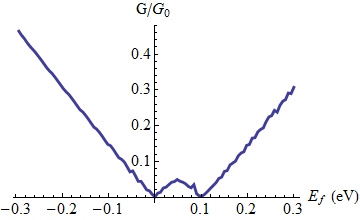
\includegraphics[scale=0.35]{images/pot-g-1}}
				\caption{$t=20$ K.}
			\end{subfigure}
			\hspace{0.5cm}
			\begin{subfigure}[h]{0.3\textwidth}
				\centerline{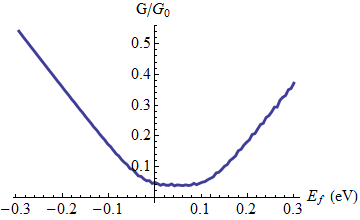
\includegraphics[scale=0.35]{images/pot-g-2}}
				\caption{$t=298$ K.}
			\end{subfigure}
			\hspace{0.5cm}
			\begin{subfigure}[h]{0.3\textwidth}
				\centerline{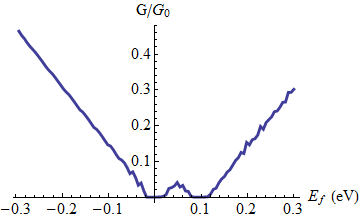
\includegraphics[scale=0.35]{images/pot-g-3}}
				\caption{$t=20$ K, $m_{a,b}=0.02$ eV.}
			\end{subfigure}
			\caption{Conductance against Fermi energy from Equation (\ref{introduction-g-t}) with the transmission probability in Equation (\ref{eq:transmission}). For all plots $V_{b}=0.1$ eV, $d=200$ nm and $eV_{sd}=0.01$ eV.}
			\label{pot-g-1}
		\end{figure}

	The height of the potential barrier is then adjusted in Figure \ref{pot-vg-1}, which would be caused by doping or interactions with a substrate. Figure \ref{pot-vg-1} (a) and Figure \ref{pot-vg-1} (b) show the dependence on barrier height at low temperatures. In Figure \ref{pot-vg-1} (a) the barrier height $V_{b}$ is adjusted, which shows oscillations caused by Fabry-P\'{e}rot resonances and an asymmetry between positive and negative gate voltages. In Figure \ref{pot-vg-1} (b) $V_{b}$ is kept constant at zero electron volts and the potential outside of region $b$ is adjusted to create a potential well or negative barrier. This shows very different results; the maximum conductance appears at zero gate voltage as with Figure \ref{pot-vg-1} (a), however, the conductance drops quickly as the sides of the well increase in height. Again there appears to be an asymmetry between the positive and negative gate voltages with negative voltages causing a sharp drop in conductance. In Figure \ref{pot-vg-1} (c) the conductance is then shown at room temperature ($298$ K). The overall conductance has increased, again with a maximum at zero gate voltage and an asymmetry between positive and negative gate voltages.
		\begin{figure}[h]
			 \begin{subfigure}[h]{0.3\textwidth}
				\centerline{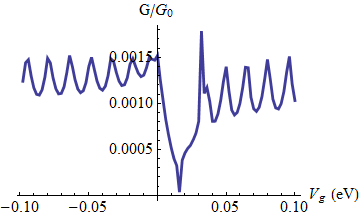
\includegraphics[scale=0.35]{images/pot-vg-1}}
				\caption{$t=20$ K, $V_{b}=V_{g}$, $V_{a}=0$ eV.}
			\end{subfigure}
			\hspace{0.5cm}
			\begin{subfigure}[h]{0.3\textwidth}
				\centerline{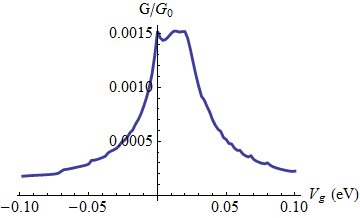
\includegraphics[scale=0.35]{images/pot-vg-2}}
				\caption{$t=20$ K, $V_{a}=V_{g}$, $V_{b}=0$ eV.}
			\end{subfigure}
			\hspace{0.5cm}
			\begin{subfigure}[h]{0.3\textwidth}
				\centerline{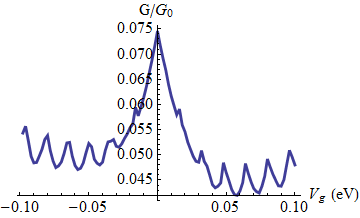
\includegraphics[scale=0.35]{images/pot-vg-3}}
				\caption{$t=298$ K, $V_{b}=V_{g}$, $V_{a}=0$ eV.}
			\end{subfigure}
			\caption{Conductance against barrier height from Equation (\ref{introduction-g-t}) with the transmission probability in Equation (\ref{eq:transmission}). For all plots $d=200$ nm and $eV_{sd}=0.01$ eV.}
			\label{pot-vg-1}
		\end{figure}

	The conductance dependence on temperature is further examined in Figure \ref{pot-t-1}. At higher temperatures the dependence becomes linear, however at lower temperatures some differing properties can be observed. When $V_{b}$ is adjusted the conductance with respect to temperature increases faster then when $V_{a}$ is adjusted, corresponding to the higher conductances shown in Figure \ref{pot-vg-1} (a) and Figure \ref{pot-t-1} (b). When an energy gap is included in the spectrum the conductance is reduced significantly becoming close to zero. At higher temperatures the charge carriers have enough energy to escape the energy gap and the linear dependence is seen again.
		\begin{figure}[h]
			 \begin{subfigure}[h]{0.3\textwidth}
				\centerline{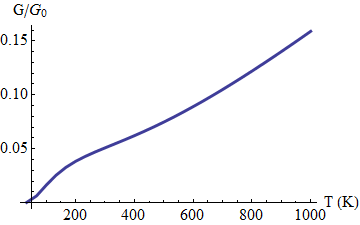
\includegraphics[scale=0.35]{images/pot-t-1}}
				\caption{$V_{b}=0.1$ eV, $V_{a}=0$ eV.}
			\end{subfigure}
			\hspace{0.5cm}
			\begin{subfigure}[h]{0.3\textwidth}
				\centerline{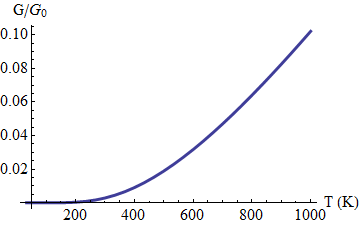
\includegraphics[scale=0.35]{images/pot-t-2}}
				\caption{$V_{b}=0.1$ eV, $V_{a}=0$ eV, $m_{a,b}=0.1$ eV.}
			\end{subfigure}
			\hspace{0.5cm}
			\begin{subfigure}[h]{0.3\textwidth}
				\centerline{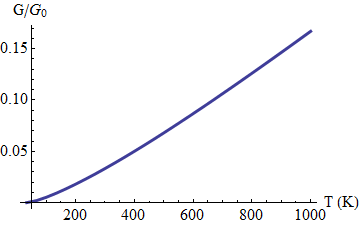
\includegraphics[scale=0.35]{images/pot-t-3}}
				\caption{$V_{a}=0.1$ eV, $V_{b}=0$ eV.}
			\end{subfigure}
			\caption{Conductance against temperature from Equation (\ref{introduction-g-t}) with the transmission probability in Equation (\ref{eq:transmission}). For all plots $d=200$ nm and $eV_{sd}=0.01$ eV.}
			\label{pot-t-1}
		\end{figure}

	By adjusting the source-drain voltage through a potential barrier the conductance becomes similar to that of a semiconducting diode. Figure \ref{pot-vsd-1} shows the conductance dependence on source-drain voltage. By comparing the high and low temperature curves in Figure \ref{pot-vsd-1} (a) and Figure \ref{pot-vsd-1} (b) it can be seen that the current increases at lower voltages with increasing temperature. The effect of an energy gap is then shown in Figure \ref{pot-vsd-1} (c). Here a large energy gap causes the conductance to become near zero at low source-drain voltages. At higher voltages the conductance behaves similarly to the gapless case, although the gap region causes a much larger asymmetry between positive and negative voltages.
		\begin{figure}[h]
			 \begin{subfigure}[h]{0.3\textwidth}
				\centerline{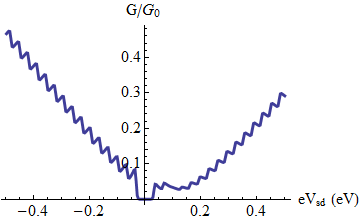
\includegraphics[scale=0.35]{images/pot-vsd-1}}
				\caption{$T=20$ K.}
			\end{subfigure}
			\hspace{0.5cm}
			\begin{subfigure}[h]{0.3\textwidth}
				\centerline{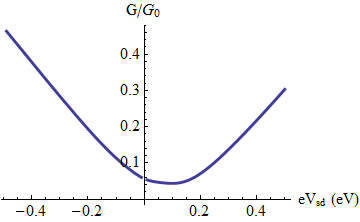
\includegraphics[scale=0.35]{images/pot-vsd-2}}
				\caption{$T=298$ K.}
			\end{subfigure}
			\hspace{0.5cm}
			\begin{subfigure}[h]{0.3\textwidth}
				\centerline{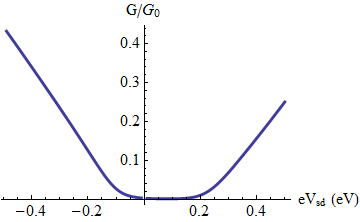
\includegraphics[scale=0.35]{images/pot-vsd-3}}
				\caption{$T=298$ K and $m_{a,b}=0.1$ eV.}
			\end{subfigure}
			\caption{Conductance against source-drain voltage from Equation (\ref{introduction-g-t}) with the transmission probability in Equation (\ref{eq:transmission}). For all plots $d=200$ nm and $V_{b}=0.1$ eV.}
			\label{pot-vsd-1}
		\end{figure}
%%%%%
%%%%%
%%%%%
		\section{Conductance Without Graphene Density of States}
		\label{Rectangular Barrier - Conductance Withount Graphene Density of States}
			If the graphene density of states is not used in the derivation for conductance, a system where graphene is only used as a scattering device can be simulated. The result for the transmission probability from Equation (\ref{eq:transmission}) can then be used to calculate the conductance through a nano-device. In this way these results will be comparable to results obtained experimentally. The conductance at zero temperature without the graphene density of states is then \cite{b4, b13, b16}:
			\begin{equation}
				G=G_{0}\int^{\pi/2}_{-\pi/2}T\left(E_{f},\theta_{a}\right)\cos(\theta_{a})d\theta_{a}
				\label{g}
			\end{equation}
			where $G_{0}=2e^{2}/\hbar$ and $E_{f}$ is the Fermi energy. Figure \ref{rectangular-barrier-conductance-a} and Figure \ref{rectangular-barrier-conductance-c} then show the conductance for various barriers where energy gap and potential have been included within defined regions. From this, the effect of the energy gap is clearly shown as the conductance sharply decreases to zero within this region. When comparing the potential barriers it can also be seen that the overall conductance decreases and oscillations become more defined as the energy gap increases. In Figure \ref{rectangular-barrier-conductance-c} (b) a single conductance curve is examined. In this figure the energies at which the peaks of the bound states occur (from Equation (\ref{boundstates})) have been included as dashed lines. It can then be seen that the troughs in conductance approximately coincide with these energies. With this in mind the energies half way between the bound states were also included as solid lines. These solid lines then approximately show the energies at which the peaks in the conductance occur.
\begin{figure}
	\begin{subfigure}{0.45\textwidth}
		\centerline{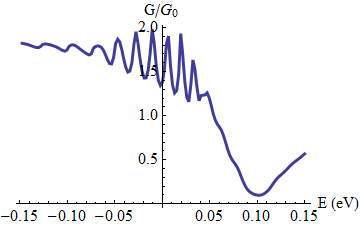
\includegraphics[scale=0.6]{images/rectangular-barrier-conductance-a}}
		\caption{$V_{b}=0.1$ eV.}
	\end{subfigure}
	\hspace{1.2cm}
	\begin{subfigure}{0.45\textwidth}
		\centerline{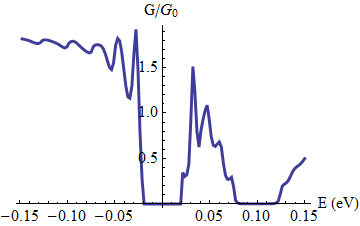
\includegraphics[scale=0.6]{images/rectangular-barrier-conductance-b}}
		\caption{$V_{b}=0.1$ eV and $m_{a,b}=0.02$ eV.}
	\end{subfigure}
	\caption{The conductance from Equation (\ref{g}) for various barriers with width $d=200$ nm.}
	\label{rectangular-barrier-conductance-a}
\end{figure}
\begin{figure}
	\begin{subfigure}{0.45\textwidth}
		\centerline{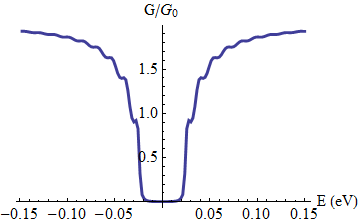
\includegraphics[scale=0.6]{images/rectangular-barrier-conductance-c}}
		\caption{$m_{b}=0.02$ eV.}
	\end{subfigure}
	\hspace{1.2cm}
	\begin{subfigure}{0.45\textwidth}
		\centerline{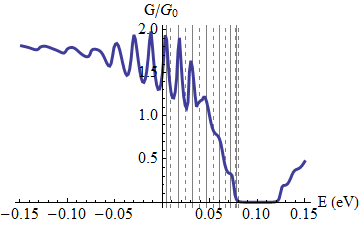
\includegraphics[scale=0.6]{images/rectangular-barrier-conductance-max}}
		\caption{$m_{a}=0$ eV, $m_{b}=0.02$ eV, $V_{a}=0$ eV and $V_{b}=0.1$ eV.}
		\label{conductance-max}
	\end{subfigure}
	\caption{The conductance from Equation (\ref{g}) for a various barriers with width $d=200$ nm. In (b) the dashed lines show peaks of the bound states from Equation (\ref{boundstates}) and solid lines are located at energies mid way between bound states.}
	\label{rectangular-barrier-conductance-c}
\end{figure}
%%%%%
%%%%%
%%%%%
			\section{n-Barriers}
			\label{Rectangular Barrier - n-Barriers}
				To adjust the transfer matrix method for multiple barriers a phase shift must be introduced for when the electron is travelling between barriers \cite{b18}. For convenience each barrier will be on its own $x$ axis, so that the first barrier starts at $x_{1}=0$ and the second barrier starts at $x_{2}=0$. The distance between the two axes will be defined as $d_{1}+l$. A diagram of the two energy axes and distance $l$ is shown in Figure \ref{n-barriers-x}.
				\begin{figure}[h]
					\centerline{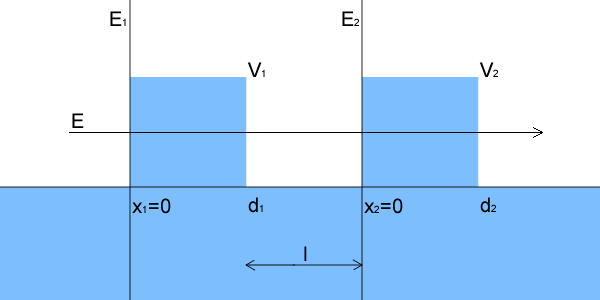
\includegraphics[scale=0.5]{images/multiple-potential-barrier-flat}}
					\caption{A double potential barrier with distance $l$ between barriers. The double barrier shown is constructed of two single potential barriers on independent axes $x_{1}$ and $x_{2}$. The two barriers can be joined by introducing a phase shift between the barriers.}
					\label{n-barriers-x}
				\end{figure}

				Continuity of the wave-functions require that the transmitted wave from the first barrier must be matched to the incident wave of the second barrier. For convenience, this will be done at the point $x_{1}=d_{1}+l/2$ and $x_{2}=-l/2$. Using the continuity of the wave-functions, which were derived in Section \ref{Wave-functions - Oscillitary}, at the points $x_{1}=d_{1}+l/2$ and $x_{2}=-l/2$ produces the relation:
				\begin{align}
					\left[\begin{array}{cc}
						e^{iq\left(d+\frac{l}{2}\right)}&e^{-iq\left(d+\frac{l}{2}\right)}\\
						\alpha_{1}e^{iq\left(d+\frac{l}{2}\right)+i\theta}&-\alpha_{1}e^{-iq\left(d+\frac{l}{2}\right)-i\theta}\\
					\end{array}\right]
					\left[\begin{array}{cc}
						a_{15}\\
						a_{16}\\
					\end{array}\right]
					&=
					\left[\begin{array}{cc}
						e^{-iq\frac{l}{2}}&e^{iq\frac{l}{2}}\\
						\alpha_{1}e^{-iq\frac{l}{2}+i\theta}&-\alpha_{1}e^{iq\frac{l}{2}-i\theta}\\
					\end{array}\right]
					\left[\begin{array}{cc}
						a_{21}\\
						a_{22}\\
					\end{array}\right]
				\end{align}
				The matrices $m_{1}$ and $m_{2}$ have been introduced to represent the wave-functions from each barrier so that:
				\begin{align}
					m_{1}
					\left[\begin{array}{cc}
						a_{15}\\
						a_{16}\\
					\end{array}\right]
					&=m_{2}
					\left[\begin{array}{cc}
						a_{21}\\
						a_{22}\\
					\end{array}\right]
				\end{align}
				Making $a_{21}$ and $a_{22}$ the subject produces the transfer matrix for the region between the two barriers:
				\begin{align}
					\left[\begin{array}{cc}
						a_{21}\\
						a_{22}\\
					\end{array}\right]
					=\Lambda
					\left[\begin{array}{cc}
						a_{15}\\
						a_{16}\\
					\end{array}\right]
					\hspace{1cm}	
					\Lambda=m_{2}^{-1}m_{1}=
					\left[\begin{array}{cc}
						e^{iq\left(d_{1}+\frac{l}{2}\right)}&0\\
						0&e^{-iq\left(d_{1}+\frac{l}{2}\right)}\\
					\end{array}\right]
				\end{align}
				Using the phase shift between the two barriers the transfer matrix for $n$ barriers can be calculated from:
				\begin{align}
					M_{n}=\Lambda^{-1}\left(\Lambda M\right)^{n}
					\label{mn}
				\end{align}

				where $M$ is the transfer matrix for a single potential barrier and $M_{n}$ is the transfer matrix for the whole barrier structure. By keeping the independent region notation from the single barrier any barrier combination can be created this way, providing there is a region between barriers. However, this can make the already complex result very unmanageable. For this reason it is convenient to use similar barriers. Some results from the evaluated transmission can be seen in Figure \ref{doubletransmissionplot}. These results show similar charateristics to the single barriers; the potential barrier shows $T=1$ when $\theta_{a}=0$ and the massive barrier contains a gap region centered at $E=0$ eV with symmetry on the energy axis. The most obvious exception is the double barrier systems show far more resonances due to the two extra wave-function regions added with the extra barrier.
\begin{figure}
	\begin{subfigure}{0.5\textwidth}
		\centerline{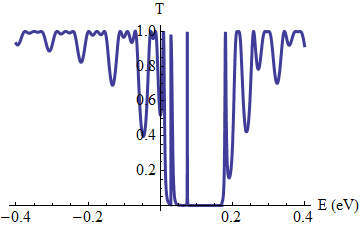
\includegraphics[scale=0.6]{images/double-potential}}
		\caption{The double potential barrier with $V_{b}=0.05$ eV.}
		\label{doubletransmissionplota}
	\end{subfigure}
	\hspace{0.6cm}
	\begin{subfigure}{0.5\textwidth}
		\centerline{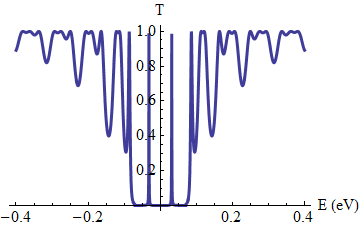
\includegraphics[scale=0.6]{images/double-mass}}
		\caption{The double mass barrier with $m_{b}=0.05$ eV.}
		\label{doubletransmissionplotb}
	\end{subfigure}
	\caption{Transmission probability for double barrier systems from the transfer matrix in Equation (\ref{mn}). For simplicity similar barriers are used where $d_{1,2}=50$ nm, $l=50$ nm and $\theta_{a}=\pi/4$.}
	\label{doubletransmissionplot}
\end{figure}

				The effect of these resonances can clearly be seen when comparing the conductance for a double barrier in Figure \ref{doubletransmissionplotg} (b) with the conductance for a single barrier in Figure \ref{rectangular-barrier-conductance-a}.
\begin{figure}
	\begin{subfigure}{0.5\textwidth}
		\centerline{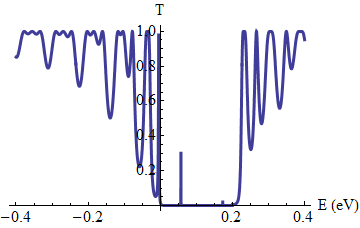
\includegraphics[scale=0.6]{images/double-potential-mass}}
		\caption{$\theta_{a}=\pi/4$.}
		\label{doubletransmissionplotga}
	\end{subfigure}
	\hspace{0.6cm}
	\begin{subfigure}{0.5\textwidth}
		\centerline{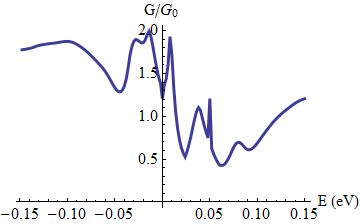
\includegraphics[scale=0.6]{images/double-potential-g}}
		\caption{}
		\label{doublegplot}
	\end{subfigure}
	\caption{(a) Transmission probability from the transfer matrix in Equation (\ref{mn}). (b) Conductance plot for symmetrical double massive potential barrier calculated from Equation (\ref{g}) with the transmission probability from the transfer matrix in Equation (\ref{mn}). For both plots the barriers have the characteristics $d_{1,2}=50$ nm, $l=50$ nm, $V_{b}=0.05$ eV and $m_{b}=0.05$ eV.}
	\label{doubletransmissionplotg}
\end{figure}
%%%%%
%%%%%
%%%%%
			\section{Graphene Superlattice}
			\label{Rectangular Barrier - Graphene Superlattice}
			The graphene superlattice consists of an infinite number of potential barriers with equal spacing. This problem can be compared to the electron in a periodic potential field \cite{b32} and is shown in Figure \ref{periodic}.
			\begin{figure}[h]
				\centerline{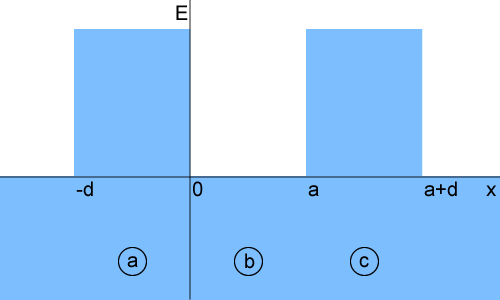
\includegraphics[scale=0.5]{images/periodic}}
				\caption{A periodic potential with distance $a$ between barriers and a barrier with $d$.}
				\label{periodic}
			\end{figure}

			The wave-functions in each region can be taken from Section \ref{Wave-functions - Oscillitary}. In region $a$ the normalised wave-functions have the form:
			\begin{align}
				\psi_{a}=
				c_{a}e^{ik_{y}y}
				\left[\begin{array}{ccc}
					e^{iq_{a}x}&e^{-iq_{a}x}\\
					\alpha_{a} e^{iq_{a}x+i\theta_{a}}&-\alpha_{a} e^{-iq_{a}x-i\theta_{a}}
				\end{array}\right]
				\left[\begin{array}{ccc}
					a_{1}\\
					a_{2}
				\end{array}\right]
			\end{align}
			In region $b$ there is no external potential and the normalised wave-functions are:
			\begin{align}
				\psi_{b}=
				c_{b}e^{ik_{y}y}
				\left[\begin{array}{ccc}
					e^{iq_{b}x}&e^{-iq_{b}x}\\
					\alpha_{b} e^{iq_{b}x+i\theta_{b}}&-\alpha_{b} e^{-iq_{b}x-i\theta_{b}}
				\end{array}\right]
				\left[\begin{array}{ccc}
					a_{3}\\
					a_{4}
				\end{array}\right]
			\end{align}
			Requiring that the potentials in regions $a$ and $c$ are the same, the wave-functions in regions $a$ and $c$ will be equivalent but with a spacial displacement and a potential phase shift of $e^{ik\left(a+d\right)}$, where $a+d$ is the period of the periodic potential. Here the constant $k=2\pi n/L$ where $L$ is the length of the entire structure and $n$ is an integer. Therefore the wave-functions can be written as:
			\begin{align}
				\psi_{c}=
				c_{a}e^{ik\left(a+d\right)}e^{ik_{y}y}
				\left[\begin{array}{ccc}
					e^{iq_{a}\left(x-a-d\right)}&e^{-iq_{a}\left(x-a-d\right)}\\
					\alpha_{a} e^{iq_{a}\left(x-a-d\right)+i\theta_{a}}&-\alpha_{a} e^{-iq_{a}\left(x-a-d\right)-i\theta_{a}}
				\end{array}\right]
				\left[\begin{array}{ccc}
					a_{1}\\
					a_{2}
				\end{array}\right]
			\end{align}
			Continuity of the wave-functions at the barrier interfaces located at $x=0$ and $x=a$ produces a set of four simultaneous equations. In matrix form these equations can be written as:
			\begin{align}
				\left[\begin{array}{cccc}
					c_{a}&c_{a}&-c_{b}&-c_{b}\\
					c_{a}\alpha_{a}e^{i\theta_{a}}&-c_{a}\alpha_{a}e^{-i\theta_{a}}&-c_{b}\alpha_{b}e^{i\theta_{b}}&c_{b}\alpha_{b}e^{-i\theta_{b}}\\
					-c_{a}e^{ik\left(a+d\right)}e^{-iq_{a}d}&-c_{a}e^{ik\left(a+d\right)}e^{iq_{a}d}&e^{iq_{b}a}&e^{-iq_{b}a}\\
					-c_{a}\alpha_{a}e^{ik\left(a+d\right)}e^{-iq_{a}d+i\theta_{a}}&c_{a}\alpha_{a}e^{ik\left(a+d\right)}e^{iq_{a}d-i\theta_{a}}&c_{b}\alpha_{b} e^{iq_{b}a+i\theta_{b}}&-c_{b}\alpha_{b} e^{-iq_{b}a-i\theta_{b}}
				\end{array}\right]
				\left[\begin{array}{cccc}
					a_{1}\\
					a_{2}\\
					a_{3}\\
					a_{4}
				\end{array}\right]
				=
				\left[\begin{array}{cccc}
					0\\
					0\\
					0\\
					0
				\end{array}\right]
			\end{align}
			These equations can be solved by requiring that the determinant of this matrix is equal to zero. Evaluating this results in the dispersion relation:
			\begin{align}
				-\sin(q_{a}d)&\sin(q_{b}d)\left[\frac{\alpha_{a}}{\alpha_{b}}+\frac{\alpha_{b}}{\alpha_{a}}\right]+\sin(q_{a}d)\sin(q_{b}d)\sin(\theta_{a})\sin(\theta_{b})\\
				&+\cos(q_{a}d)\cos(q_{b}d)\cos(\theta_{a})\cos(\theta_{b})-\cos(2kd)\cos(\theta_{a})\cos(\theta_{b})=0
				\label{Rectangular Barrier band eq}
			\end{align}
			For simplicity the widths of the periodic potential barriers and wells have been made equivalent so that $a=d$. The roots of this equation produce the energy bands of a graphene superlattice shown in Figure \ref{superlattice-bands}.
			\begin{figure}
				\begin{subfigure}{0.5\textwidth}
					\centerline{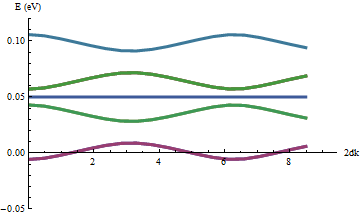
\includegraphics[scale=0.6]{images/superlattice-bands-k}}
					\caption{The energy band dependence on the phase factor $k$ with $k_{y}=0$.}
				\end{subfigure}
				\hspace{0.6cm}
				\begin{subfigure}{0.5\textwidth}
					\centerline{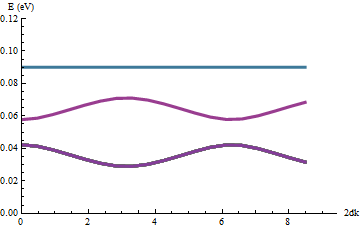
\includegraphics[scale=0.6]{images/superlattice-bands}}
					\caption{The energy band dependence on the phase factor $k$ with $k_{y}=0.01$.}
				\end{subfigure}
				\caption{The energy bands for an infinite graphene superlattice from Equation (\ref{Rectangular Barrier band eq}). The lattice shown has a height $V_{a}=0.1$ eV and the width $d=50$ nm.}
				\label{superlattice-bands}
			\end{figure}
%\end{document}